\documentclass[12pt,a4paper]{article}  % Déclare la classe du document.

\newcommand{\chaptermark}[2]{\og #2 \fg{} (#1)} % ligne uniquement pour éviter une erreur en cas d'article
\usepackage[table,dvipsnames,svgnames]{xcolor}
\usepackage{listingsutf8}
%\usepackage[utf8]{inputenc}% gestion des accents (source)
\usepackage[T1]{fontenc}% gestion des accents (PDF)
\usepackage{fontspec}
\usepackage[french]{babel}% gestion du français
\usepackage{textcomp}% caractères additionnels
\usepackage{mathtools,amssymb,amsthm}% packages de l'AMS + mathtools
\usepackage{amsmath}
\usepackage{yhmath}
\usepackage{mathpazo}
\usepackage[scaled=0.95]{helvet}
\usepackage{courier}
%\usepackage{fourier}
%\usepackage[scaled=0.95]{helvet}
%\usepackage{courier}
\usepackage{bm}
\usepackage{gensymb}
\usepackage{graphicx}

\usepackage{enumitem}
\usepackage{pifont}

\usepackage{pstricks}
\usepackage{pstricks-add}
\usepackage{pst-eucl}
\usepackage{pgfplots}
\let\clipbox\relax
%\usepackage{pst-plot,pst-text,pst-tree,pstricks-add}
%\usepackage{pst-node} % required package
\usepackage{pst-all}
\usepackage[most,skins,breakable]{tcolorbox}

\usepackage{euscript}





% ############### Nouvelles commandes ###############
% Coloration des labels des points dans pst-eucl
\makeatletter
\define@key[psset]{pst-eucl}{LabelColor}{\def\psk@LabelColor{#1}}
\psset{LabelColor=black}
\def\Pst@WhichLabel#1{{\color{\psk@LabelColor}%
		\ifx\psk@PointName\@default#1\else\psk@PointName\fi}}
\makeatother

% renomme le symbole #2 en #1#2 et invalide le symbole initial #2:
\def\renamesymbol#1#2{
	\expandafter\let\expandafter\newsym\expandafter=\csname#2\endcsname
	\expandafter\global\expandafter\let\csname#1#2\endcsname=\newsym
	\expandafter\global\expandafter\let\csname#2\endcsname=\origsym
}



\usepackage{ProfCollege}
\renamesymbol{Casio}{Calculatrice}
\usepackage[nonshellescape]{ProfLycee}



%\usepackage[left=1.5cm,right=1.5cm,top=2.5cm,bottom=2.5cm]{geometry}
\usepackage[left=13mm,right=13mm,top=18mm,bottom=18mm,footskip=30pt]{geometry}
\setlength{\headheight}{15pt}

\usepackage{titlesec}
\usepackage{pas-math}
\usepackage{longtable}
\usepackage{tikz,tkz-tab}
\usepackage{amsmath}
\usepackage[right]{eurosym}
\usepackage{sectsty}
\usepackage{tipfr}
\usepackage{setspace}

%pour faire les touches de la calculatrices
\usepackage{menukeys}
\renewmenumacro{\menu}{roundedmenus} % default: menus
\renewmenumacro{\directory}{pathswithfolder} % default: paths
\renewmenumacro{\keys}{shadowedroundedkeys} % default: roundedkeys


\usepackage{multicol}
\usepackage{multirow}
\usepackage{systeme}

%% Format des titres de chapitres, paragraphes, ...
\titleformat{\chapter}[frame]
{\color{red!85!white}\normalsize}%
{\filright\sffamily\Large%
	\enspace Chapitre \thechapter\enspace}%
{8pt}
{\color{red!85!white}\rule{0pt}{30pt}\sffamily\Huge\bfseries\filcenter}
%%%%%%%%%%%%%%%%%%%%
\titlespacing{\chapter}{0pc}{0pc}{2pc}
\titlespacing{\subsection}{2pc}{}{}

\titleformat{\subsection}[block]{\hspace{1em}}{\thesubsection}{1em .}{}
\titleformat{\subsubsection}[block]{\hspace{2em}}{\thesubsection}{1em )}{}

\chapterfont{\color{red}{}}
\sectionfont{\color{green!55!black}{}}
\subsectionfont{\color{cyan!65!black}{}}
\subsubsectionfont{\color{violet}{}}
\renewcommand{\thesection}{\color{green!55!black}\Roman{section}.}
\renewcommand{\thesubsection}{\color{cyan!65!black}\arabic{subsection})}
\renewcommand{\thesubsubsection}{\color{violet}\alph{subsubsection})}
\setcounter{secnumdepth}{3}

\titleformat{\subsection}[block]{\hspace{1em}}{\thesubsection}{1em .}{}
\titleformat{\subsubsection}[block]{\hspace{2em}}{\thesubsection}{1em )}{}

\usepackage[column=A]{cellspace}
\setlength{\cellspacebottomlimit}{4pt}
\setlength{\cellspacetoplimit}{4pt}
\setlength{\parindent}{2pt}
\setlength{\tabcolsep}{0.5cm}


%entête et pieds de pages
\usepackage{fancyhdr}
\pagestyle{fancy}
\fancyhf{}
\usepackage{lastpage}
\renewcommand{\chaptermark}[1]{\markboth {Chap. \thechapter~ - ~#1}{}}
\renewcommand\headrulewidth{1pt}
\fancyhead[LO,RE]{1ère G - spécialité maths}
\fancyhead[RO,LE]{\leftmark}
\renewcommand\footrulewidth{1pt}
\fancyfoot[LO,RE]{Année 2025-2026}
\fancyfoot[RO,LE]{\textbf{Page \thepage/\pageref{LastPage}}}

%Mes boites pour les définitions, propriétés, remarques, ...

%Mes boites pour les définitions, propriétés, remarques, ...

\newcommand\titrebox[1]{\textbf{#1}}
\newtcolorbox{definition}{breakable,colback=red!10!white,
	colframe=red!85!white, fonttitle=\bfseries,enhanced,
	attach boxed title to top left={xshift=5mm, yshift=-2mm},boxed title style={size=small,colback=red!10!white,colframe=red!85!white, arc=0.5mm},
	title=\textcolor{red!85!white}{Définition} , arc=3mm}

\newtcolorbox{definitionTitre}[1]{breakable,colback=red!10!white,
	colframe=red!85!white, fonttitle=\bfseries,enhanced,
	attach boxed title to top left={xshift=5mm, yshift=-2mm},boxed title style={size=small,colback=red!10!white,colframe=red!85!white, arc=0.5mm},
	title=\textcolor{red!85!white}{Définition - #1} , arc=3mm}

\newtcolorbox{definitionPerso}[1]{breakable,colback=red!10!white,
	colframe=red!85!white, fonttitle=\bfseries,enhanced,
	attach boxed title to top left={xshift=5mm, yshift=-2mm},boxed title style={size=small,colback=red!10!white,colframe=red!85!white, arc=0.5mm},
	title=\textcolor{red!85!white}{#1} , arc=3mm}

\newtcolorbox{regle}{breakable,colback=red!10!white,
	colframe=red!85!white, fonttitle=\bfseries,enhanced,
	attach boxed title to top left={xshift=5mm, yshift=-2mm},boxed title style={size=small,colback=red!10!white,colframe=red!85!white, arc=0.5mm},
	title=\textcolor{red!85!white}{Règle} , arc=3mm}

\newtcolorbox{regles}{breakable,colback=red!10!white,
	colframe=red!85!white, fonttitle=\bfseries,enhanced,
	attach boxed title to top left={xshift=5mm, yshift=-2mm},boxed title style={size=small,colback=red!10!white,colframe=red!85!white, arc=0.5mm},
	title=\textcolor{red!85!white}{Règles} , arc=3mm}

\newtcolorbox{definitions}{breakable,colback=red!10!white,
	colframe=red!85!white, fonttitle=\bfseries,enhanced,
	attach boxed title to top left={xshift=5mm, yshift=-2mm},boxed title style={size=small,colback=red!10!white,colframe=red!85!white, arc=0.5mm},
	title=\textcolor{red!85!white}{Définitions} , arc=3mm}

\newtcolorbox{propriete}{breakable,colback=red!10!white,
	colframe=red!85!white, fonttitle=\bfseries,enhanced,
	attach boxed title to top left={xshift=5mm, yshift=-2mm},boxed title style={size=small,colback=red!10!white,colframe=red!85!white, arc=0.5mm},
	title=\textcolor{red!85!white}{Propriété} , arc=3mm}

\newtcolorbox{proprieteTitre}[1]{breakable,colback=red!10!white,
	colframe=red!85!white, fonttitle=\bfseries,enhanced,
	attach boxed title to top left={xshift=5mm, yshift=-2mm},boxed title style={size=small,colback=red!10!white,colframe=red!85!white, arc=0.5mm},
	title=\textcolor{red!85!white}{Propriété - #1} , arc=3mm}

\newtcolorbox{proprietes}{breakable,colback=red!10!white,
	colframe=red!85!white, fonttitle=\bfseries,enhanced,
	attach boxed title to top left={xshift=5mm, yshift=-2mm},boxed title style={size=small,colback=red!10!white,colframe=red!85!white, arc=0.5mm},
	title=\textcolor{red!85!white}{Propriétés} , arc=3mm}

\newtcolorbox{theoreme}{breakable,colback=red!10!white,
	colframe=red!85!white, fonttitle=\bfseries,enhanced,
	attach boxed title to top left={xshift=5mm, yshift=-2mm},boxed title style={size=small,colback=red!10!white,colframe=red!85!white, arc=0.5mm},
	title=\textcolor{red!85!white}{Théorème} , arc=3mm}

\newtcolorbox{theoremeTitre}[1]{breakable,colback=red!10!white,
	colframe=red!85!white, fonttitle=\bfseries,enhanced,
	attach boxed title to top left={xshift=5mm, yshift=-2mm},boxed title style={size=small,colback=red!10!white,colframe=red!85!white, arc=0.5mm},
	title=\textcolor{red!85!white}{Théorème - #1} , arc=3mm}

\newtcolorbox{theoremes}{breakable,colback=red!10!white,
	colframe=red!85!white, fonttitle=\bfseries,enhanced,
	attach boxed title to top left={xshift=5mm, yshift=-2mm},boxed title style={size=small,colback=red!10!white,colframe=red!85!white, arc=0.5mm},
	title=\textcolor{red!85!white}{Théorèmes} , arc=3mm}

\newtcolorbox{bexemple}{
	enhanced,
	breakable,
	fonttitle=\bfseries,
	frame empty,
	nobeforeafter,
	borderline west={0.5mm}{0mm}{cyan!75!black},
	title=\textcolor{cyan!75!black}{\faHubspot\:\:Exemple},
	%title after break=Exemple (suite),
	colback=white,
	extras={enhanced, frame empty},
	detach title,before upper={\tcbtitle\ :\quad },
}

\newtcolorbox{bexemples}{
	enhanced,
	breakable,
	fonttitle=\bfseries,
	frame empty,
	nobeforeafter,
	borderline west={0.5mm}{0mm}{cyan!75!black},
	title=\textcolor{cyan!75!black}{\faHubspot\:\:Exemples},
	%title after break=Exemples (suite),
	colback=white,
	extras={enhanced, frame empty},
	detach title,before upper={\tcbtitle\ :\quad },
}

\newtcolorbox{bexemplet}[1]{
	enhanced,
	breakable,
	fonttitle=\bfseries,
	frame empty,
	borderline west={0.5mm}{0mm}{cyan!75!black},
	title=\textcolor{cyan!75!black}{\faHubspot\:\:Exemple - #1},
	colback=white,
	extras={enhanced, frame empty},
	detach title,before upper={\tcbtitle\ :\quad },
}

\newtcolorbox{brmq}{
	enhanced,
	breakable,
	fonttitle=\bfseries,
	frame empty,
	nobeforeafter,
	borderline west={0.5mm}{0mm}{orange!95!white},
	title=\textcolor{orange!85!white}{\faHandPointRight[regular]\:\:Remarque} ,
	colback=white,
	extras={enhanced, frame empty},
	detach title,before upper={\tcbtitle\ \quad },
}

\newtcolorbox{brmqs}{
	enhanced,
	breakable,
	fonttitle=\bfseries,
	frame empty,
	nobeforeafter,
	borderline west={0.5mm}{0mm}{orange!85!white},
	title=\textcolor{orange!85!white}{\faHandPointRight[regular]\:\:Remarques},
	colback=white,
	detach title,before upper={\tcbtitle\ \quad },
	extras={enhanced, frame empty},
}

\newtcolorbox{brmqt}[1]{
	enhanced,
	breakable,
	fonttitle=\bfseries,
	frame empty,
	nobeforeafter,
	borderline west={0.5mm}{0mm}{orange!85!white},
	title=\textcolor{orange!85!white}{\faHandPointRight[regular]\:\:Remarque - #1},
	colback=white,
	extras={enhanced, frame empty},
	detach title,before upper={\tcbtitle\ \quad },
}

\newtcolorbox{consequences}[1]{
	enhanced,
	breakable,
	fonttitle=\bfseries,
	frame empty,
	nobeforeafter,
	borderline west={0.5mm}{0mm}{ProcessBlue},
	title=\textcolor{ProcessBlue}{#1},
	colback=white,
	extras={enhanced, frame empty},
	detach title,before upper={\tcbtitle\ :\quad },
}

\newtcolorbox{bmethode}{
	enhanced,
	breakable,
	fonttitle=\bfseries,
	frame empty,
	nobeforeafter,
	borderline west={0.5mm}{0mm}{blue!75!black},
	title=\textcolor{blue!75!black}{Méthode} ,
	colback=white,
	extras={enhanced, frame empty},
	attach boxed title to top left = {xshift = -3mm},
	boxed title style={size=small,colback=white,colframe=blue!75!black, arc=3mm,
	}
}

\newtcolorbox{bmethodes}{
	enhanced,
	breakable,
	fonttitle=\bfseries,
	frame empty,
	nobeforeafter,
	borderline west={0.5mm}{0mm}{blue!75!black},
	title=\textcolor{blue!75!black}{Méthodes} ,
	colback=white,
	extras={enhanced, frame empty},
	attach boxed title to top left = {xshift = -3mm},
	boxed title style={size=small,colback=blue!75!black,colframe=blue!75!black, arc=3mm,
	}
	boxed title after break style={size=small,colback=white,colframe=blue!75!black, arc=3mm,
	}
}

\newtcolorbox{bmethodet}[1]{
	enhanced,
	breakable,
	fonttitle=\bfseries,
	frame empty,
	nobeforeafter,
	borderline west={0.5mm}{0mm}{blue!75!black},
	title=\textcolor{blue!75!black}{\faTasks\:\:Méthode - #1} ,
	colback=white,
	extras={enhanced, frame empty},
	attach boxed title to top left = {xshift = -3mm},
	boxed title style={size=small,colback=white,colframe=blue!75!black, arc=3mm,
	}
}

\newtcolorbox{bdemo}{
	enhanced,
	breakable,
	fonttitle=\bfseries,
	frame empty,
	nobeforeafter,
	borderline west={0.5mm}{0mm}{violet!65!white},
	title={\faEdit[regular]\:\:Démonstration},
	%title after break=Démonstration (suite),
	colback=white,
	extras={enhanced, frame empty},
	attach boxed title to top left = {xshift = -3mm},
	boxed title style={size=small,colback=violet!65!white,colframe=violet!65!white, arc=3mm,
	}
}

\newtcolorbox{bdemos}{
	enhanced,
	breakable,
	fonttitle=\bfseries,
	frame empty,
	nobeforeafter,
	borderline west={0.5mm}{0mm}{violet!65!white},
	title={\faEdit[regular]\:\:Démonstrations},
	%title after break=Démonstration (suite),
	colback=white,
	extras={enhanced, frame empty},
	attach boxed title to top left = {xshift = -3mm},
	boxed title style={size=small,colback=violet!65!white,colframe=violet!65!white, arc=3mm,
	}
}

\newtcolorbox{bdemot}[1]{
	enhanced,
	breakable,
	fonttitle=\bfseries,
	frame empty,
	nobeforeafter,
	borderline west={0.5mm}{0mm}{violet!65!white},
	title={\faEdit[regular]\:\:Démonstration - #1},
	%title after break=Démonstration (suite),
	colback=white,
	extras={enhanced, frame empty},
	attach boxed title to top left = {xshift = -3mm},
	boxed title style={size=small,colback=violet!65!white,colframe=violet!65!white, arc=3mm,
	}
}

\newtcolorbox{boxPerso}[2]{
	enhanced,
	breakable,
	fonttitle=\bfseries,
	frame empty,
	nobeforeafter,
	borderline west={0.5mm}{0mm}{#2},
	title=#1,
	%title after break=Exemple (suite),
	colback=white,
	extras={enhanced, frame empty},
	detach title,before upper={\tcbtitle\ :\quad },
}


\newcommand*{\Coord}[3]{% 
	\ensuremath{\vv{#1}\, 
		\begin{pmatrix} 
			#2\\ 
			#3 
\end{pmatrix}}}

\newcommand*{\CoordSV}[2]{% 
	\ensuremath{\begin{pmatrix} 
			#1\\ 
			#2 
\end{pmatrix}}}

\newcommand*{\Coordp}[3]{% 
	\ensuremath{\vv{#1}\, 
		\left\lvert 
		\begin{matrix} 
			#2\\ 
			#3 
		\end{matrix}  
		\right.% Ne pas oublier le délimiteur invisible. 
}}


%personnalisation des listes non numérotées pour les différentes boites 
\newlist{itemEx}{itemize}{2}
\setlist[itemEx,1]{label=$\bullet$, font=\color{cyan!75!black}}
\setlist[itemEx,2]{label=$\bullet$, font=\color{cyan!75!black}}

\newlist{enumEx}{enumerate}{2}
\setlist[enumEx,1]{label=\arabic*), font=\bf\color{cyan!75!black}}
\setlist[enumEx,2]{label=\alph*), font=\bf\color{cyan!75!black}}

\newlist{itemMet}{itemize}{2}
\setlist[itemMet,1]{label=$\bullet$, font=\color{blue!75!black}}
\setlist[itemMet,2]{label=$\bullet$, font=\color{blue!75!black}}

\newlist{enumMet}{enumerate}{2}
\setlist[enumMet,1]{label=\arabic*), font=\bf\color{blue!75!black}}
\setlist[enumMet,2]{label=\alph*), font=\bf\color{blue!75!black}}

\newlist{itemDef}{itemize}{2}
\setlist[itemDef,1]{label=$\bullet$, font=\color{ForestGreen}}
\setlist[itemDef,2]{label=$\bullet$, font=\color{ForestGreen}}

\newlist{enumDef}{enumerate}{2}
\setlist[enumDef,1]{label=\arabic*), font=\bf\color{ForestGreen}}
\setlist[enumDef,2]{label=\alph*), font=\bf\color{ForestGreen}}

\newlist{itemProp}{itemize}{2}
\setlist[itemProp,1]{label=$\bullet$, font=\color{red!85!white}}
\setlist[itemProp,2]{label=$\bullet$, font=\color{red!85!white}}

\newlist{enumProp}{enumerate}{2}
\setlist[enumProp,1]{label=\arabic*), font=\bf\color{red!85!white}}
\setlist[enumProp,2]{label=\alph*), font=\bf\color{red!85!white}}

\newlist{itemDem}{itemize}{2}
\setlist[itemDem,1]{label=$\bullet$, font=\color{violet!85!white}}
\setlist[itemDem,2]{label=$\bullet$, font=\color{violet!85!white}}

\newlist{enumDem}{enumerate}{2}
\setlist[enumDem,1]{label=\arabic*), font=\bf\color{violet!85!white}}
\setlist[enumDem,2]{label=\alph*), font=\bf\color{violet!85!white}}

\newlist{itemRem}{itemize}{2}
\setlist[itemRem,1]{label=\ding{43}, font=\color{orange!85!white}}
\setlist[itemRem,2]{label=\ding{43}, font=\color{orange!85!white}}

\newlist{enumRem}{enumerate}{2}
\setlist[enumRem,1]{label=\arabic*), font=\bf\color{orange!85!white}}
\setlist[enumRem,2]{label=\alph*), font=\bf\color{orange!85!white}}

% nouvelle commande pour mettre entre guillemets une expression
\newcommand{\guillemets}[1]{\og \emph{#1} \fg}


\newcommand{\corr}[1]{\fcolorbox{red}{yellow!30}{#1}}

\newtcolorbox{corrBox}{enhanced,breakable,boxrule=1pt,nobeforeafter,boxsep=0pt,left=\fboxsep,right=\fboxsep,colback=yellow!30,colframe=red!75!black}

% commandes pour mettre en couleur (et en gras) dans une expression mathématique.
\newcommand{\mVert}[1]{{\color{green!55!black}\bm{#1}}}
\newcommand{\mVertWB}[1]{{\color{green!55!black}#1}}
\newcommand{\mRouge}[1]{{\color{red!85!white}\bm{#1}}}
\newcommand{\mRougeWB}[1]{{\color{red!85!white}#1}}
\newcommand{\mBleu}[1]{{\color{blue!75!black}\bm{#1}}}
\newcommand{\mBleuWB}[1]{{\color{blue!75!black}#1}}
\newcommand{\mOrange}[1]{{\color{orange!75!white}\bm{#1}}}
\newcommand{\mOrangeWB}[1]{{\color{orange!75!white}#1}}
\newcommand{\mViolet}[1]{{\color{violet!85!white}\bm{#1}}}
\newcommand{\mVioletWB}[1]{{\color{violet!85!white}#1}}

%commandes pour les flèches de distributivité.
\newcommand{\tikzmarkBB}[2][]{ \tikz[remember picture, overlay, baseline=-0.5ex]\node[#1, left](#2){}; }
\newcommand{\flechePropV}[4][]{ \tikz[remember picture, overlay]\draw (#2)edge[bend left=90,min distance=1em, -stealth]node[midway, #1]{#4}(#3); }
\newcommand{\flechePropH}[4][]{ \tikz[remember picture, overlay]\draw (#2)edge[bend left=90, min distance=1em, -stealth]node[midway, #1]{#4}(#3); }
\newcommand{\flechePropHbas}[4][]{ \tikz[remember picture, overlay]\draw (#2)edge[bend left=-90, min distance=1em, -stealth]node[midway, #1]{#4}(#3); }


\lstdefinestyle{algo}{%
	inputencoding=utf8,
	mathescape,
	basicstyle=\footnotesize\ttfamily,
	numberstyle=\scriptsize\ttfamily\color{gray},
	showstringspaces=false,
	tabsize=2,
	numbers=left,
	framexleftmargin=8mm,
	xleftmargin=8mm,
	keepspaces=true,
	frame=lines,
	framerule=1pt,
	rulecolor=\color{green!50!black},
	backgroundcolor=\color{green!5},
	keywords = {Pour, allant, Si, alors, Sinon, Fin},    
	morecomment=[l][commentstyle]{//},
	commentstyle=\color{gray},
	classoffset=0,
	keywordstyle=\color{blue!75},
	classoffset=1,
	morekeywords = {Afficher},
	keywordstyle=\color{green!50!black},
	classoffset=0,
	morestring=[b]",
	stringstyle=\color{red!75},
	literate=
	{é}{{\'e}}{1}%
	{è}{{\`e}}{1}%
	{à}{{\`a}}{1}%
	{â}{{\^a}}{1}%%%
	{ç}{{\c{c}}}{1}%
	{œ}{{\oe}}{1}%
	{ù}{{\`u}}{1}%
	{É}{{\'E}}{1}%
	{È}{{\`E}}{1}%
	{À}{{\`A}}{1}%
	{Ç}{{\c{C}}}{1}%
	{Œ}{{\OE}}{1}%
	{Ê}{{\^E}}{1}%
	{ê}{{\^e}}{1}%
	{î}{{\^i}}{1}%
	{ï}{{\"i}}{1}%%%
	{ô}{{\^o}}{1}%
	{û}{{\^u}}{1}%
	{=}{$\leftarrow$}{1}%
	{==}{$={}$}{1}}


%  --------   Macro pour les exercices et leur numérotation  

\newcounter{exo}

\setcounter{exo}{1}

\newcommand{\exercice}[1]{\vskip 0.2cm\noindent{\bf \ Exercice \theexo {  #1 }}\addtocounter{exo}{1}}

\newcounter{rit}

\setcounter{rit}{1}

\newcommand{\rituel}[1]{\vskip 0.2cm\noindent{ \bf \ \underline{Rit. \therit {  #1 }}}\addtocounter{rit}{1}}

\newcommand{\raisedrule}[2][0em]{\leaders\hbox{\rule[#1]{1pt}{#2}}\hfill}

\newcounter{numexo}

\setcounter{numexo}{1}

\newcommand{\exerciceDS}[1]{\vskip 0.6cm\noindent\rule[+2pt]{1cm}{0.5pt}\ {\large\bf \ Exercice \thenumexo {  #1 }}\raisedrule[+2pt]{0.5pt}\null\addtocounter{numexo}{1}\par\vskip 0,4cm}

\newcommand{\bareme}[1]{\tikz\node[circle,draw,inner sep=1pt,outer sep=1pt, color=red]{\textbf{#1}};}

%  --------   Pour le langage Python

% Default fixed font does not support bold face
\DeclareFixedFont{\ttb}{T1}{txtt}{bx}{n}{12} % for bold
\DeclareFixedFont{\ttm}{T1}{txtt}{m}{n}{12}  % for normal

% Custom colors
\usepackage{color}
\definecolor{deepblue}{rgb}{0,0,0.5}
\definecolor{deepred}{rgb}{0.6,0,0}
\definecolor{deepgreen}{rgb}{0,0.5,0}

\usepackage{listings}

% Python style for highlighting
\newcommand\pythonstyle{\lstset{
		language=Python,
		basicstyle=\ttm,
		otherkeywords={self},             % Add keywords here
		keywordstyle=\ttb\color{deepblue},
		emph={MyClass,__init__},          % Custom highlighting
		emphstyle=\ttb\color{deepred},    % Custom highlighting style
		stringstyle=\color{deepgreen},
		frame=tb,                         % Any extra options here
		showstringspaces=false            % 
}}


% Python environment
\lstnewenvironment{python}[1][]
{
	\pythonstyle
	\lstset{#1}
}
{}

% Python for external files
\newcommand\pythonexternal[2][]{{
		\pythonstyle
		\lstinputlisting[#1]{#2}}}

% Python for inline
\newcommand\pythoninline[1]{{\pythonstyle\lstinline!#1!}}


% \begin{document}
	
	% \section{``In-text'' listing highlighting}
	
	% \begin{python}
		% class MyClass(Yourclass):
		%     def __init__(self, my, yours):
		%         bla = '5 1 2 3 4'
		%         print bla
		% \end{python}
	
	% \section{External listing highlighting}
	
	% \pythonexternal{demo.py}
	
	% \section{Inline highlighting}
	
	% Definition \pythoninline{class MyClass} means \dots
	
	% \end{document}

\definecolor{codegreen}{rgb}{0,0.6,0}
\definecolor{codegray}{rgb}{0.5,0.5,0.5}
\definecolor{codepurple}{rgb}{0.58,0,0.82}
\definecolor{backcolour}{rgb}{0.95,0.95,0.92}

\lstdefinestyle{myStyle}{
	backgroundcolor=\color{backcolour},   
	commentstyle=\color{codegreen},
	keywordstyle=\color{magenta},
	numberstyle=\tiny\color{codegray},
	stringstyle=\color{codepurple},
	basicstyle=\ttfamily\footnotesize,
	breakatwhitespace=false,         
	breaklines=true,                 
	captionpos=b,                    
	keepspaces=true,                 
	numbers=left,                    
	numbersep=5pt,                  
	showspaces=false,                
	showstringspaces=false,
	showtabs=false,                  
	tabsize=2
}

\lstset{style=myStyle}

\newcommand{\normeB}[1]{\left\Vert \vv{#1}\right\Vert}

\newcommand\grasmaths[1]{\symbf{#1}}
\newcommand\sfbmath[1]{\symbf{\symsfup{#1}}}
\definecolor{marron}{rgb}{0.64,0.16,0.16}
\definecolor{titrebleu}{rgb}{0,0,0.6}

\usepackage{tabularx}
\usepackage{wasysym}
% ===========================tableaux de base
\newcolumntype{R}[1]{>{\raggedleft\arraybackslash }b{#1}} 
\newcolumntype{L}[1]{>{\raggedright\arraybackslash }b{#1}}
\newcolumntype{C}[1]{>{\centering\arraybackslash }b{#1}}
\newcolumntype{M}[1]{>{\centering\arraybackslash }m{#1}} %doublecentrée
\renewcommand{\tabularxcolumn}[1]{m{#1}}
\newcolumntype{Y}{>{\centering\arraybackslash }X}

%=============================boîtes de cours
\usepackage{fontawesome5}
\newcommand\fontbox{\sffamily}
%\newcommand\titrebox[1]{\textbf{#1}}
\tcbuselibrary{breakable}
\tcbset{bdefaut/.style={%
		fonttitle=\fontbox,%
		enhanced,breakable,center,boxrule=1.25pt,drop shadow=black!33!white,%
		sharp corners=uphill,arc=12pt,before skip=12pt,after skip=12pt,%
		left=5pt,leftupper=5pt,top=1mm,bottom=1mm,%
		before upper=\leavevmode
	}
}
\NewDocumentCommand\bbnewbox{ m m m m O{#4} !O{} }{%nom + titre + icone + bordure/titre/fondtitre + couleur fond + options
	\DeclareTColorBox{#1}{ O{} }{%
		bdefaut,%
		colframe=#4,coltitle=#4!25!Black,colbacktitle=#4!35,colback=#5!10,%
		title={#3\:\:\titrebox{#2##1}},%
		#6
	}%
}

\bbnewbox{bdefi}{Définition}{\faIcon[regular]{comment-dots}}{ForestGreen}
\bbnewbox{bcor}{Corollaire}{\faIcon[regular]{comment-dots}}{ForestGreen}
\bbnewbox{bdefis}{Définitions}{\faIcon[regular]{comment-dots}}{ForestGreen}
\bbnewbox{bhumour}{Humour}{\faIcon[regular]{laugh-wink}}{Yellow}
%\bbnewbox{bprop}{Propriété}{\faCog}{Salmon}
\bbnewbox{bprop}{Propriété}{\faCog}{red!85!white}
\bbnewbox{bprops}{Propriétés}{\faCog}{Salmon}
\bbnewbox{bcscq}{Conséquence}{\faArrowAltCircleRight[regular]}{Salmon}
\bbnewbox{bthm}{Théorème}{\faBullhorn}{FireBrick}
\bbnewbox{blog}{Logiciel}{\faDev}{CornflowerBlue}[white]
\bbnewbox{bhistoire}{Point histoire}{\faUniversity}{Chocolate}[white]

%\bbnewbox{brmq}{Remarque}{\faHandPointRight[regular]}{MidnightBlue}[white]
\bbnewbox{bexercice}{Exercice}{\faHubspot}{MidnightBlue}
%\bbnewbox{bexemple}{Exemple}{\faHubspot}{MediumTurquoise}
\bbnewbox{bvoc}{Vocabulaire}{\faList*[regular]}{YellowGreen}
\bbnewbox{bnota}{Notation}{\faList*}{YellowGreen}
\bbnewbox{bregle}{Règle}{\faList*}{YellowGreen}
\bbnewbox{bcadre}{Cadre}{\faInfoCircle}{Peru}
\bbnewbox{bidee}{Idée}{\faInfo}{LightBlue}
\bbnewbox{bintro}{Intro}{\faMarker}{LightSalmon}
\bbnewbox{billustr}{Illustration}{\faChartLine}{Crimson}[White]
\bbnewbox{bvideo}{}{\faIcon[regular]{file-video}}{teal}[White]
\bbnewbox{bbilan}{Bilan}{\faForward}{Purple}
%\bbnewbox{bmethode}{Méthode}{\faTasks}{Coral}
%\bbnewbox{bmethode}{Méthode}{\faTasks}{blue!75!black}
\bbnewbox{btuto}{Tuto}{\faTerminal}{Coral}[White]
\bbnewbox{bmanip}{Manipulation}{\faCodeBranch}{DarkCyan}[White]
\bbnewbox{bcalco}{Calculatrice}{\faCalculator}{MediumVioletRed}[White]
\bbnewbox{boutil}{Outil}{\faTools}{DeepSkyBlue}[White]
\bbnewbox{basavoir}{À savoir}{\faHeart}{Red}
\bbnewbox{bbloctd}{TD}{\faHourglassStart}{LightSeaGreen}[White]
\bbnewbox{bblocdm}{À vous de jouer}{\faHourglassStart}{LightSeaGreen}[White]
%\bbnewbox{brappel}{Rappel}{\faHandPointUp[regular]}{LightSalmon}
\bbnewbox{brappel}{Rappel}{\faHandPointUp[regular]}{Peru}
\bbnewbox{bresol}{Résolution}{\faPuzzlePiece}{LightSeaGreen}[White]
\bbnewbox{battention}{Attention}{\faExclamationTriangle}{Red}
\bbnewbox{bcode}{Code}{\faCode}{Crimson}[White]
\bbnewbox{bpython}{Python}{\faPython}{SeaGreen}[White]

\newcommand{\grasInDef}[1]{\textcolor{ForestGreen!55!black}{\textbf{#1}}}
\newcommand{\grasInProp}[1]{\textcolor{red!85!white}{\textbf{#1}}}
\newcommand{\grasInEx}[1]{\textcolor{MediumTurquoise!55!black}{\textbf{#1}}}
\newcommand{\grasInRem}[1]{\textcolor{orange!65!white}{\textbf{#1}}}
\newcommand{\grasInMet}[1]{\textcolor{blue!75!black}{\textbf{#1}}}
\newcommand{\grasInDem}[1]{\textcolor{violet!85!white}{\textbf{#1}}}

%\newtcolorbox{bmethodet}[1][]{%
%	bdefaut,%
%	colframe=blue!75!black,coltitle=white,colbacktitle=blue!65!black,colback=blue!75!black!15!white,
%	title={\faTasks\:\:\titrebox{{Méthode - #1}}}
%}

%outil
\newtcolorbox{boutilcalc}[1][]{%
	bdefaut,%
	colframe=DeepSkyBlue,coltitle=black,colbacktitle=DeepSkyBlue!35,colback=White,
	title=\textcolor{DeepSkyBlue!25!Black}{\faFileVideo[regular]\:\:\titrebox{Tuto#1 Vidéo}}
}

%loglogo
\newtcolorbox{bloglogo}[2][]{%
	bdefaut,%
	colframe=CornflowerBlue,coltitle=black,colbacktitle=CornflowerBlue!35,colback=white,
	title=\textcolor{CornflowerBlue!25!Black}{\faDev\:\:\titrebox{Logiciel#1}},
	overlay={\begin{tcbclipinterior}
			\node[opacity=0.33,rotate=-45] at ($(interior.south east)+(-10pt,10pt)$){\includegraphics[height=24pt]{#2}};
	\end{tcbclipinterior}}
}

%demo
%\newtcolorbox{bdemo}[1][]{%
%	bdefaut,%
%	colframe=Violet,coltitle=black,colbacktitle=Violet!35,colback=Violet!15,
%	title=\textcolor{Violet!25!Black}{\faEdit[regular]\:\:\titrebox{Démonstration#1}},
%	overlay={\begin{tcbclipinterior}%
%			\node[] at ($(interior.south east)+(-10pt,10pt)$){\large\textcolor{Violet}{\textbf{\CheckedBox}}};%
%	\end{tcbclipinterior}}
%}


%\newtcolorbox{bdemo}[1][]{%
%	bdefaut,%
%	colframe=violet!85!white,coltitle=black,colbacktitle=Violet!35,colback=Violet!15,
%	title=\textcolor{Violet!25!Black}{\faEdit[regular]\:\:\titrebox{Démonstration#1}},
%	overlay={\begin{tcbclipinterior}%
%			\node[] at ($(interior.south east)+(-10pt,10pt)$){\large\textcolor{Violet}{\textbf{\CheckedBox}}};%
%	\end{tcbclipinterior}}
%}

%demoblanc
\newtcolorbox{bdemoblanc}[1][]{%
	bdefaut,%
	colframe=Violet,coltitle=black,colbacktitle=Violet!35,colback=White,
	title=\textcolor{Violet!25!Black}{\faEdit[regular]\:\:\titrebox{Démonstration#1}},
	overlay={\begin{tcbclipinterior}%
			\node[] at ($(interior.south east)+(-10pt,10pt)$){\large\textcolor{Violet}{\textbf{\CheckedBox}}};%
	\end{tcbclipinterior}}
}

%algo
\newtcolorbox{balgo}[1][]{%
	bdefaut,%
	colframe=OrangeRed,coltitle=black,colbacktitle=OrangeRed!35,colback=White,
	title=\textcolor{OrangeRed!25!Black}{\faFileCode\:\:\titrebox{Algorithme#1}},
	overlay={\begin{tcbclipinterior}%
			\node[opacity=0.15,rotate=-15] at ($(interior.south east)+(-8pt,12pt)$){\includegraphics[height=24pt]{algorithmvec}};%
	\end{tcbclipinterior}}
}


%aide
\newtcolorbox{baide}{%
	bdefaut,%
	colframe=titrebleu!35,coltitle=titrebleu!50!Black,colbacktitle=titrebleu!15,colback=White,
	title=\textcolor{titrebleu!25!Black}{\faBacon\:\:\titrebox{Niveaux de difficulté}},
	overlay={\begin{tcbclipinterior}%
			\node[opacity=0.33,rotate=45,scale=0.33] at ($(interior.south east)+(-6pt,6pt)$){\textcolor{titrebleu!50!Black}{\footnotesize \bfseries \sffamily \textcopyright{} Dairon11}};%
	\end{tcbclipinterior}}
}

\newtcolorbox{bcalcologo}[2][]{%
	bdefaut,%
	colframe=MediumVioletRed,coltitle=black,colbacktitle=MediumVioletRed!35,colback=White,
	title=\textcolor{MediumVioletRed!25!Black}{\faCalculator\:\:\titrebox{Calculatrice#1}},
	overlay={\begin{tcbclipinterior}%
			\node[opacity=0.33,rotate=-45] at ($(interior.south east)+(-10pt,10pt)$){\includegraphics[height=48pt]{#2}};%
	\end{tcbclipinterior}}
}

\definecolor{orangescratch}{HTML}{F8A31F}
\newtcolorbox{bscratch}[1][]{%
	bdefaut,%
	colframe=orangescratch,coltitle=black,colbacktitle=orangescratch!35,colback=White,
	title=\textcolor{orange!25!Black}{\includegraphics[height=1em]{scratch}\:\:\titrebox{Scratch#1}},
	overlay={\begin{tcbclipinterior}%
			\node[opacity=0.33,rotate=45] at ($(interior.south east)+(-12pt,12pt)$){\includegraphics[height=12pt]{scratchban}};%
	\end{tcbclipinterior}}
}

%reponse
\newtcolorbox{breponse}[1][]{%
	bdefaut,%
	colframe=Thistle,coltitle=black,colbacktitle=Thistle!35,colback=White,
	before upper = \vspace{-0.05cm},
	title=\textcolor{Thistle!25!Black}{\faIcon{pen-alt}\:\:\titrebox{Réponse#1}}
}

\usepackage{dashundergaps}
\newcommand\underdash[1][black]{% <- règle la couleur du texte
	\bgroup
	\ifdim\ULdepth=\maxdimen\settodepth\ULdepth{(j}\advance\ULdepth.4pt\fi
	\markoverwith{\kern0.2em% <- règle l'espacement avant un pointillé
		\vtop{\kern0.5ex% <- règle l'altitude des pointillés
			{\color{black}% <- règle la couleur des pointillés
				\hrule width.4em% <- règle la largeur des pointillés
		}}\kern0.2em% <- règle l'espacement après un pointillé
	}\color{#1}\ULon}

\newcommand\pointille[1][1cm]{\makebox[#1]{\dotfill}}



\usepackage{epic}   % extension et simplification de  l'environnement picture
\usepackage{graphicx}    % permet d'inclure des graphique externe dans un document
\usepackage{arydshln}   %permet d'avoir des lignes en pointillés

\newcommand{\lignes}[1]{
\setlength{\unitlength}{1mm}
\vskip 0,4cm\noindent
\multido{\i=0+1}{#1}{%
     \noindent
     \begin{picture}(150,5)
     \linethickness{0,005mm}
     \put(-5,0){\dashline{1}(175,5)(5,5)}
     \end{picture}\vskip 0,001cm
     }
\vskip 0cm
}

\rhead{\textcolor{red}{Correction - Fiche d'exercices - Appl. Produit Scalaire}}

\begin{document}
\graphicspath{{images/}}

\begin{center}
\fbox{
\begin{minipage}[]{15cm}
\begin{center}
\LARGE{\rule{0.5cm}{0pt}\rule[-0.25cm]{0pt}{0.9cm}
\textcolor{red}{Correction - Fiche d'exercices}\\
Application produit scalaire
}
\end{center}
\end{minipage}
}

\end{center}


% \begin{center}\textbf{2h - Calculatrice autorisée - Barème indicatif}\end{center}

% %\begin{center}\textbf{Les élèves avec un tier-temps ne traitent pas les questions avec  le symbole \ding{46}}\end{center}

% \begin{center}
% %On veillera à ENCADRER ses résultats et soigner sa copie.\\
% Les résultats doivent être justifiés par des calculs (au moins 1 étape intermédiaire).
% \end{center}

\exerciceDS{}
$\mathrm{ABC}$ est un triangle tel que :$A B=2, A C=6 \text { et } \widehat{B A C}=60^{\circ} .$\\
Calculer la valeur exacte de la longueur $B C$.

\begin{corrBox}
$\vv{AB}\cdot\vv{AC}=AB\times AC\times\cos(\widehat{BAC})=2\times6\times\cos(60)=6$\\
On a également :\\
$\vv{AB}\cdot\vv{AC}=\dfrac{1}{2}(AB^2+AC^2-BC^2)$\\
Soit : $BC^2=AB^2+AC^2-2\vv{AB}\cdot\vv{AC}$\\
Donc : $BC^2=2^2+6^2-2\times6=28$\\
D'ou $BC=\sqrt{28}=2\sqrt{7}$
\end{corrBox}

\exerciceDS{}
ABCD est un parallélogramme tel que :$A B=6, A D=4 \text { et } \widehat{D A B}=60^{\circ} .$
%\begin{multicols}{2}
\begin{enumMet}
    \item Construire une figure.\\
    \begin{corrBox}
        \newrgbcolor{ududff}{0.30196078431372547 0.30196078431372547 1.}
        \newrgbcolor{xdxdff}{0.49019607843137253 0.49019607843137253 1.}
        \newrgbcolor{qqwuqq}{0. 0.39215686274509803 0.}
        \psset{xunit=1.0cm,yunit=1.0cm,algebraic=true,dimen=middle,dotstyle=o,dotsize=5pt 0,linewidth=1.6pt,arrowsize=3pt 2,arrowinset=0.25}
        \begin{pspicture*}(-2.28,7)(22.12,12.02)
        \psline[linewidth=2.pt](3.,8.)(9.,8.)
        \pscustom[linewidth=2.pt,linecolor=qqwuqq,fillcolor=qqwuqq,fillstyle=solid,opacity=0.1]{
        \parametricplot{0.0}{1.0471975511965976}{0.6*cos(t)+3.|0.6*sin(t)+8.}
        \lineto(3.,8.)\closepath}
        \psline[linewidth=2.pt](3.,8.)(5.,11.464101615137757)
        \psline[linewidth=2.pt](5.,11.464101615137757)(11.,11.464101615137757)
        \psline[linewidth=2.pt](11.,11.464101615137757)(9.,8.)
        \begin{scriptsize}
        %\psdots[dotstyle=*,linecolor=ududff](3.,8.)
        \rput[bl](2.6,7.66){\ududff{$A$}}
        %\psdots[dotstyle=*,linecolor=xdxdff](9.,8.)
        \rput[bl](8.94,7.48){\xdxdff{$B$}}
        \rput[bl](5.98,7.7){$6$}
        \rput[bl](3.68,8.26){\qqwuqq{$\alpha = 60^{\circ}$}}
        %\psdots[dotsize=4pt 0,dotstyle=*,linecolor=darkgray](5.,11.464101615137757)
        \rput[bl](4.78,11.72){\darkgray{$D$}}
        %\psdots[dotsize=4pt 0,dotstyle=*,linecolor=darkgray](11.,11.464101615137757)
        \rput[bl](11.38,11.62){\darkgray{$C$}}
        \rput[bl](3.56,9.8){$4$}
        \end{scriptsize}
        \end{pspicture*}
    \end{corrBox}
    \item Calculer la longueur BD.\\
    \begin{corrBox}
        $\vv{AB}\cdot\vv{AD}=AB\times AD\times\cos(\widehat{BAD})=6\times4\times\cos(60)=12$\\
        $\vv{A B} \cdot \vv{A D}=\dfrac{1}{2}\left(A B^{2}+A D^{2}-B D^{2}\right)$\\
        $12=\dfrac{1}{2}\left(6^{2}+4^{2}-B D^{2}\right)$\\
        $24=36+16-BD^2$\\
        $BD^2=28$\\
        $BD=\sqrt{28}=2\sqrt{7}$
    \end{corrBox}
    \item Quelle est la mesure de l'angle $\widehat{A B C}$ ?\\
    \begin{corrBox}
        Dans un quadrilatère la somme des angles fait $360^{\circ}$.\\
        De plus dans un parallélogramme, les côtés opposés sont égaux.\\
        Donc $\widehat{ABC}=\dfrac{1}{2}(360-2\times60)=120^{\circ}$
    \end{corrBox}   
    \item Calculer la longueur AC.\\
    \begin{corrBox}
        $\vv{BA}\cdot\vv{BC}=AB\times BC\times\cos(\widehat{ABC})=6\times4\times\cos(120)=-12$\\
        $\vv{BA} \cdot \vv{BC}=\dfrac{1}{2}\left(BA^{2}+BC^{2}-AC^{2}\right)$\\
        $-12=\dfrac{1}{2}\left(6^{2}+4^{2}-AC^{2}\right)$\\
        $-24=36+16-AC^2$\\
        $AC^2=76$\\
        $AC=\sqrt{76}$
    \end{corrBox}
\end{enumMet}
%\end{multicols}

\vspace{-0.3cm}
\exerciceDS{}

\begin{minipage}[c]{0.55\linewidth}
Un voilier V approche de la côte. Il est situé à 9 milles du phare A, à 5 milles du phare $B$ et l'angle $\widehat{AVB}$ mesure $60^{\circ} .$
Calculer la distance AB entre les deux phares. Arrondir au dixième.
\end{minipage} \hfill
\begin{minipage}[c]{0.4\linewidth}
\begin{center}
    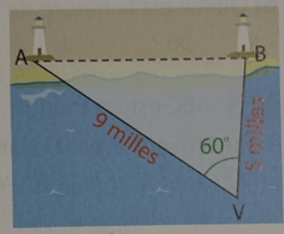
\includegraphics[scale=0.9]{images/1.06.04 - Img01.png}
\end{center}
\end{minipage}

\begin{corrBox}
    $\vv{VA}\cdot\vv{VB}=VA\times VB\times\cos(\widehat{AVB})=9\times5\times\cos(60)=22,5$\\
    $\vv{VA} \cdot \vv{VB}=\dfrac{1}{2}\left(VA^{2}+VB^{2}-AB^{2}\right)$\\
    $22,5=\dfrac{1}{2}\left(9^{2}+5^{2}-AB^{2}\right)$\\
    $45=81+25-AB^2$\\
    $AB^2=61$\\
    $AB=\sqrt{61}\approx7,8$
\end{corrBox}

\exerciceDS{}
Dans les 2 cas ci dessous, calculer $\vv{A B} \cdot \vv{A C}$.
\begin{multicols}{2}
\begin{enumMet}
    \item \ \\
    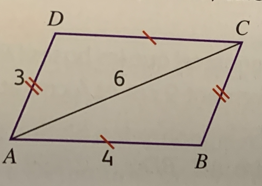
\includegraphics[scale=1.2]{images/1.06.04 - Img02.png}\\
    \begin{corrBox}
        $\vv{AB}\cdot\vv{AC}=\dfrac{1}{2}(AB^2+AC^2-BC^2)=\dfrac{1}{2}(4^2+6^2-3^2)=21,5$
    \end{corrBox}
    \columnbreak
    \item \ \\
    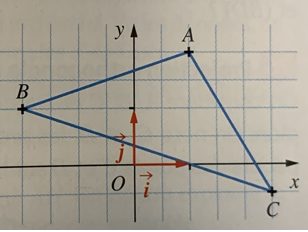
\includegraphics[scale=1.2]{images/1.06.04 - Img03.png}\\
    \begin{corrBox}
        $\vv{AB}\cdot\vv{AC}=xx'+yy'=-3\times1,5+(-1)\times(-2,5)=-2$
    \end{corrBox}
\end{enumMet}
\end{multicols}

\exerciceDS{}
On considère deux vecteurs $\vv{u}$ et $\vv{v}$ du plan tels que $\|\vv{u}+\vv{v}\|=5$ et $\|\vv{u}-\vv{v}\|=3$. Calculer le produit scalaire $\vv{u} \cdot \vv{v}$.\\

\begin{corrBox}
    $\vv{u} \cdot \vv{v}=\dfrac{1}{4}\left(\|\vv{u}+\vv{v}\|^{2}-\|\vv{u}-\vv{v}\|^{2}\right)=\dfrac{1}{4}\times(5^2-3^2)=\dfrac{1}{4}\times16=4$
\end{corrBox}

\exerciceDS{}
Dans le plan muni d'un repère orthonormé, on considère les vecteurs
$\Coord{u}{2}{-3}$ et $\Coord{v}{1}{2}$.
\begin{enumMet}
    \item calculer $\vv{u} \cdot \vv{v},\|\vv{u}\|$ et $\|\vv{v}\|$.\\
    \begin{corrBox}
        $\vv{u}\cdot\vv{v}=2\times1-3\times2=-4$, $\left\|\vv{u}\right\|=\sqrt{2^2+(-3)^2}=\sqrt{13}$ et $\left\|\vv{v}\right\|=\sqrt{1^2+2^2}=\sqrt{5}$
    \end{corrBox}
    \item Calculer de deux façons les nombres : $\|\vv{u}+\vv{v}\|^{2} \text { et }\|\vv{u}-\vv{v}\|^{2}$\\
    \begin{corrBox}
        \fbox{$\left\|\vv{u}+\vv{v}\right\|^2$}\\
        \grasInMet{1ère méthode:}\\
        On sait que $\vv{u} \cdot \vv{v}=\dfrac{1}{2}\left(\|\vv{u}+\vv{v}\|^{2}-\|\vv{u}\|^{2}-\|\vv{v}\|^{2}\right)$ donc:\\
        $\|\vv{u}+\vv{v}\|^{2}=2\vv{u} \cdot \vv{v}+\|\vv{u}\|^{2}+\|\vv{v}\|^{2}=2\times(-4)+13+5=10$\\
        \grasInMet{2ème méthode:}\\
        $\Coord{u}{2}{-3}+\Coord{v}{1}{2}=\vv{u}+\vv{v} \CoordSV{3}{-1}$\\
        $\|\vv{u}+\vv{v}\|^{2}=3^2+(-1)^2=10$\\
        \ \\
        \fbox{$\left\|\vv{u}-\vv{v}\right\|^2$}\\
        \grasInMet{1ère méthode:}\\
        On sait que $\vv{u} \cdot \vv{v}=\dfrac{1}{2}\left(\|\vv{u}\|^{2}+\|\vv{v}\|^{2}-\|\vv{u}-\vv{v}\|^{2}\right)$ donc:\\
        $\|\vv{u}-\vv{v}\|^{2}=\|\vv{u}\|^{2}+\|\vv{v}\|^{2}-2\vv{u} \cdot \vv{v}=13+5-2\times(-4)=26$\\
        \grasInMet{2ème méthode:}\\
        $\Coord{u}{2}{-3}-\Coord{v}{1}{2}=\vv{u}-\vv{v} \CoordSV{1}{-5}$\\
        $\|\vv{u}-\vv{v}\|^{2}=1^2+(-5)^2=26$
    \end{corrBox}
    \item Calculer de deux façons $(\vv{u}+\vv{v}) \cdot(\vv{u}-\vv{v})$.\\
    \begin{corrBox}
        \grasInMet{1ère méthode:}\\
            $(\vv{u}+\vv{v}) \cdot(\vv{u}-\vv{v})=\|\vv{u}\|^{2}-\|\vv{v}\|^{2}=13-5=8$\\
        \grasInMet{2ème méthode:}\\
        $\vv{u}+\vv{v} \CoordSV{3}{-1} \cdot \vv{u}-\vv{v} \CoordSV{1}{-5}=3\times1+(-1)\times(-5)=8$
    \end{corrBox}
    
\end{enumMet}

\exerciceDS{}
Le plan est muni d'un repère orthonormé. Dans chaque cas, calculer $\vv{A B} \cdot \vv{A C}$ puis une mesure (arrondie au degré près) de l'angle $\widehat{B A C}$.
\begin{enumMet}
    \item $A(-1 ; 4), B(2 ; 2)$ et $C(1 ; 5)$\\
    \begin{corrBox}
        $\Coord{AB}{x_B-x_A}{y_B-y_A}=\Coord{AB}{2-(-1)}{2-4}=\Coord{AB}{3}{-2} \Longrightarrow AB=\sqrt{3^2+(-2)^2}=\sqrt{13}$\\
        $\Coord{AC}{x_C-x_A}{y_C-y_A}=\Coord{AC}{1-(-1)}{5-4}=\Coord{AC}{2}{1} \Longrightarrow AC=\sqrt{2^2+1^2}=\sqrt{5}$\\
        $\Coord{BC}{x_C-x_B}{y_C-y_B}=\Coord{BC}{1-2}{5-2}=\Coord{BC}{-1}{3} \Longrightarrow BC=\sqrt{(-1)^2+3^2}=\sqrt{10}$\\
        $\vv{A B} \cdot \vv{A C}=3\times2+(-2)\times1=4$\\
        $\vv{A B} \cdot \vv{A C}=AB\times AC\times\cos(\widehat{B A C})$\\
        $4=\sqrt{13}\times\sqrt{5}\times\cos(\widehat{B A C})$\\
        $\widehat{B A C}=\cos^{-1}\left(\dfrac{4}{\sqrt{13}\times\sqrt{5}}\right)\approx60^{\circ}$
    \end{corrBox}
    \item $A(2 ; 4), B(1 ; 3)$ et $C(4 ; 2)$\\
    \begin{corrBox}
        $\Coord{AB}{x_B-x_A}{y_B-y_A}=\Coord{AB}{1-2}{3-4}=\Coord{AB}{-1}{-1} \Longrightarrow AB=\sqrt{(-1)^2+(-1)^2}=\sqrt{2}$\\
        $\Coord{AC}{x_C-x_A}{y_C-y_A}=\Coord{AC}{4-2}{2-4}=\Coord{AC}{2}{-2} \Longrightarrow AC=\sqrt{2^2+(-2)^2}=\sqrt{8}$\\
        $\Coord{BC}{x_C-x_B}{y_C-y_B}=\Coord{BC}{4-1}{2-3}=\Coord{BC}{3}{-1} \Longrightarrow BC=\sqrt{3^2+(-1)^2}=\sqrt{10}$\\
        $\vv{A B} \cdot \vv{A C}=(-1)\times2+(-1)\times(-2)=0$\\
        donc $\widehat{B A C}=90^{\circ}$
    \end{corrBox}
    \item $A(0 ; 4), B(-3 ; 5)$ et $C(6 ; 2)$\\
    \begin{corrBox}
        $\Coord{AB}{x_B-x_A}{y_B-y_A}=\Coord{AB}{-3-0}{5-4}=\Coord{AB}{-3}{1} \Longrightarrow AB=\sqrt{(-3)^2+1^2}=\sqrt{10}$\\
        $\Coord{AC}{x_C-x_A}{y_C-y_A}=\Coord{AC}{6-0}{2-4}=\Coord{AC}{6}{-2} \Longrightarrow AC=\sqrt{6^2+(-2)^2}=\sqrt{40}$\\
        $\Coord{BC}{x_C-x_B}{y_C-y_B}=\Coord{BC}{6-(-3)}{2-5}=\Coord{BC}{9}{-3} \Longrightarrow BC=\sqrt{9^2+(-3)^2}=\sqrt{90}$\\
        $\vv{A B} \cdot \vv{A C}=-3\times6+1\times(-2)=-20$\\
        $\vv{A B} \cdot \vv{A C}=AB\times AC\times\cos(\widehat{B A C})$\\
        $-20=\sqrt{10}\times\sqrt{40}\times\cos(\widehat{B A C})$\\
        $-20=20\times\cos(\widehat{B A C})$\\
        $\widehat{B A C}=\cos^{-1}\left(-1\right)=180^{\circ}$
    \end{corrBox}
\end{enumMet}


\exerciceDS{}
Dans un repère orthonormé du plan, on considère les points $A(1 ; 4), B(-3 ;-2)$ et $C(2 ;-5)$.\\
Déterminer les angles du triangle $A B C$ à 0,1 degré près.\\
\begin{corrBox}
    On utilise le théorème d'AL-Kashi : Dans un triangle $\mathrm{ABC},$ on a, avec les notations de la figure :
    $$
    a^{2}=b^{2}+c^{2}-2 b c \cos \hat{A} \iff \hat{A}=\cos^{-1}\left(\dfrac{b^2+c^2-a^2}{2bc}\right)
    $$
    \begin{center}
        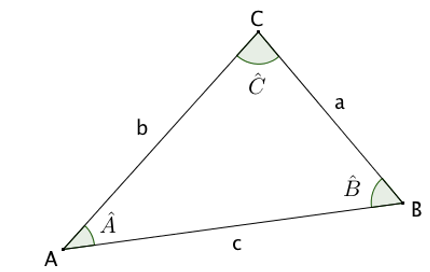
\includegraphics[scale=0.7]{1.04.IMG-03}
    \end{center}
    On commence donc par calculer les 3 longueurs:\\
    $\Coord{AB}{x_B-x_A}{y_B-y_A}=\Coord{AB}{-3-1}{-2-4}=\Coord{AB}{-4}{-6} \Longrightarrow AB=\sqrt{(-4)^2+(-6)^2}=\sqrt{52}$\\
    $\Coord{AC}{x_C-x_A}{y_C-y_A}=\Coord{AC}{2-1}{-5-4}=\Coord{AC}{1}{-9} \Longrightarrow AC=\sqrt{1^2+(-9)^2}=\sqrt{82}$\\
    $\Coord{BC}{x_C-x_B}{y_C-y_B}=\Coord{BC}{2-(-3)}{-5-(-2)}=\Coord{BC}{5}{-3} \Longrightarrow BC=\sqrt{5^2+(-3)^2}=\sqrt{34}$\\
    On peut maintenant calculer les angles:\\
    $\widehat{BAC}=\cos^{-1}\left(\dfrac{AC^2+AB^2-BC^2}{2\times AC\times AB}\right)=\cos^{-1}\left(\dfrac{82+52-34}{2\times \sqrt{82}\times \sqrt{52}}\right)\approx40,0^{^\circ}$\\
    $\widehat{ABC}=\cos^{-1}\left(\dfrac{BC^2+AB^2-AC^2}{2\times BC\times AB}\right)=\cos^{-1}\left(\dfrac{34+52-82}{2\times \sqrt{34}\times \sqrt{52}}\right)\approx87,3^{^\circ}$\\
    $\widehat{ACB}=180-\widehat{BAC}-\widehat{ABC}=180-40-87,3=52,7^{^\circ}$
\end{corrBox}

\exerciceDS{}
$A B C$ est un triangle tel que $A B=4, A C=3$ et $\widehat{B A C}=135^{\circ} . M$ est le milieu du segment $[A C]$ et $P$ est le point déini par $\vv{A P}=\dfrac{3}{4} \vv{A B}$.
\begin{enumMet}
    \item En notant que $\vv{M P}=\vv{A P}-\vv{A M}$, calculer $\vv{M P}^2$.\\
    \begin{corrBox}
        $\vv{M P}^2=(\vv{A P}-\vv{A M})^2=\vv{A P}^2-2\vv{A P}\cdot\vv{A M}+\vv{A M}^2=\vv{A P}^2-2\times \dfrac{3}{4}\times\dfrac{1}{2}\vv{A B}\cdot\vv{A C}+\vv{A M}^2$\\
        $\vv{M P}^2=3^2-\dfrac{3}{4}\times3\times4\times\cos(135)+1,5^2=\dfrac{18\sqrt{2}+45}{4}$
    \end{corrBox}
    \item En déduire la longueur $M P$.\\
    \begin{corrBox}
        $MP^2=\dfrac{18\sqrt{2}+45}{4} \iff MP=\sqrt{\dfrac{18\sqrt{2}+45}{4}}\approx4,2$
    \end{corrBox}
\end{enumMet}

\exerciceDS{}
$A B C D$ est un parallélogramme tel que $A B=3$, $A D=5$ et $A C=6$.
\begin{enumMet}
    \item 1. Rappeler la formule exprimant $\vv{u} \cdot \vv{v}$ en fonction de $\|\vv{u}\|,\|\vv{v}\|$ et $\|\vv{u}+\vv{v}\|$.\\
    Calculer alors le produit scalaire $\vv{A B} \cdot \vv{A D}$.\\
    \begin{corrBox}
        On sait que $\vv{u} \cdot \vv{v}=\dfrac{1}{2}\left(\|\vv{u}+\vv{v}\|^{2}-\|\vv{u}\|^{2}-\|\vv{v}\|^{2}\right)$ donc\\
        $\vv{AB} \cdot \vv{AD}=\dfrac{1}{2}\left(\|\vv{AB}+\vv{AD}\|^{2}-\|\vv{AB}\|^{2}-\|\vv{AD}\|^{2}\right)=\dfrac{1}{2}(6^2-5^2-3^2)=1$
    \end{corrBox}   
    \item En déduire une mesure, en degré, de l'angle $\widehat{B A D}$ (on donnera une valeur arrondie au degré près).\\
    \begin{corrBox}
        $\vv{AB}\cdot\vv{AD}=AB\times AD\times\cos(\widehat{BAD})$\\
        $1=3\times5\times\cos(\widehat{BAD})$\\
        $\widehat{BAD}=\cos^{-1}\left(\dfrac{1}{15}\right)\approx86\degree$
    \end{corrBox}
\end{enumMet}

\exerciceDS{}
$A B C D$ est un parallélogramme tel que $A B=4$, $A D=6$ et $\widehat{B A D}=40^{\circ}$.\\
Calculer le produit scalaire $\vv{A B} \cdot \vv{A C}$ (on pourra décomposer le vecteur $\vv{A C}$ ).

\begin{corrBox}
\newrgbcolor{qqwuqq}{0. 0.39215686274509803 0.}
\psset{xunit=1.0cm,yunit=1.0cm,algebraic=true,dimen=middle,dotstyle=o,dotsize=5pt 0,linewidth=2.pt,arrowsize=3pt 2,arrowinset=0.25}
\begin{pspicture*}(-0.78,-0.54)(11,4.5)
\pspolygon[linewidth=2.pt,linecolor=red,fillcolor=red,fillstyle=solid,opacity=0.1](1.,1.)(4.06,3.57)(10.06,3.57)(7.,1.)
\pscustom[linewidth=2.pt,linecolor=qqwuqq,fillcolor=qqwuqq,fillstyle=solid,opacity=0.1]{
\parametricplot{0.0}{0.6981317007977319}{0.6*cos(t)+1.|0.6*sin(t)+1.}
\lineto(1.,1.)\closepath}
\begin{scriptsize}
\rput[bl](0.66,1.14){\large{$A$}}
\rput[bl](6.78,1.2){\large{$D$}}
\rput[bl](1.7,1.14){\large{\qqwuqq{$\alpha = 40^{\circ}$}}}
\rput[bl](3.98,3.88){\large{$B$}}
\rput[bl](9.92,3.74){\large{$C$}}
\rput[bl](2.78,2.16){\large{\red{AB = 4}}}
\rput[bl](4.04,1.18){\large{\red{AD = 6}}}
\end{scriptsize}
\end{pspicture*}

$\vv{A B} \cdot \vv{A C}=\vv{A B} \cdot (\vv{A D}+\vv{DC})$\\
$\phantom{\vv{A B} \cdot \vv{A C}}=\vv{A B} \cdot (\vv{A D}+\vv{AB})$\\
$\phantom{\vv{A B} \cdot \vv{A C}}=\vv{A B} \cdot \vv{A D} + \vv{A B} \cdot \vv{A B}$\\
$\phantom{\vv{A B} \cdot \vv{A C}}=AB\times AD\times\cos(\widehat{BAD}) + AB\times AB$\\
$\phantom{\vv{A B} \cdot \vv{A C}}=4\times 6\times\cos(40) + 4\times 4$\\
$\phantom{\vv{A B} \cdot \vv{A C}}\approx34,4$
\end{corrBox}





\end{document}

